\chapter{Matriisit}

Matriisi on kaksiulotteinen taulukko,
jolle on määritelty laskutoimituksia.
Tässä luvussa näemme, miten matriisien
avulla voi optimoida dynaamista ohjelmointia.
Osoittautuu, että jos dynaamisen ohjelmoinnin rekursiossa
lasketaan yhteen kiinteä määrä aiempia arvoja
vakiokertoimilla,

\section{Laskutoimitukset}

\textit{Matriisi} on
kaksiulotteista taulukkoa
vastaava matemaattinen käsite,
jolle on määritelty laskutoimituksia
samaan tapaan kuin luvuille.

Olkoon $X$ matriisi, jonka koko on $n \times m$,
missä $n$ on korkeus (rivien määrä)
ja $m$ on leveys (sarakkeiden määrä).
Merkintä $X[i,j]$ tarkoittaa matriisin alkiota,
joka on rivillä $i$ sarakkeessa $j$,
kun $1 \le i \le n$ ja $1 \le j \le m$.

Esimerkiksi matriisin
\[
A = 
 \begin{bmatrix}
  6 & 13 & 7 & 4 \\
  7 & 0 & 8 & 2 \\
  9 & 5 & 4 & 18 \\
 \end{bmatrix}
\]

koko on $3 \times 4$,
eli sen korkeus on 3 ja leveys on 4.
Esimerkiksi $A[2,3]=8$,
koska rivillä 2 sarakkeessa 3
on luku 8.

Matriisi on \textit{neliömatriisi}, jos $n=m$ eli
matriisin korkeus ja leveys ovat samat.
Esimerkiksi seuraava matriisi on neliömatriisi:

\[
A = 
 \begin{bmatrix}
  3 & 12 & 4  \\
  5 & 9 & 15  \\
  0 & 2 & 4 \\
 \end{bmatrix}
\]

\subsubsection{Yhteenlasku}

Matriisien $A$ ja $B$ yhteenlasku $A+B$ on määritelty,
jos matriisit ovat yhtä suuret.
Tuloksena on matriisi $C=A+B$,
joka on yhtä suuri kuin matriisit $A$ ja $B$.
Matriisin $C$ alkiot lasketaan kaavalla

\[ C[i,j]=A[i,j]+B[i,j]. \]

Esimerkiksi

\[
 \begin{bmatrix}
  6 & 1 & 4 \\
  3 & 9 & 2 \\
 \end{bmatrix}
+
 \begin{bmatrix}
  4 & 9 & 3 \\
  8 & 1 & 3 \\
 \end{bmatrix}
=
 \begin{bmatrix}
  6+4 & 1+9 & 4+3 \\
  3+8 & 9+1 & 2+3 \\
 \end{bmatrix}
=
 \begin{bmatrix}
  10 & 10 & 7 \\
  11 & 10 & 5 \\
 \end{bmatrix}.
\]
Matriisien yhteenlasku on vaihdannainen ja liitännäinen,
eli pätee $A+B=B+A$ ja $A+(B+C)=(A+B)+C$.
Lukua 0 vastaa nollamatriisi $O$,
jolle pätee $A+O=A$ ja $O+A=A$.
Nollamatriisin jokainen alkio on 0.
Esimerkiksi

\[
 \begin{bmatrix}
  6 & 1 & 4 \\
  3 & 9 & 2 \\
 \end{bmatrix}
+
 \begin{bmatrix}
  0 & 0 & 0 \\
  0 & 0 & 0 \\
 \end{bmatrix}
=
 \begin{bmatrix}
  6 & 1 & 4 \\
  3 & 9 & 2 \\
 \end{bmatrix}.
\]

\subsubsection{Kertolasku}

Matriisien $A$ ja $B$ kertolasku $A \cdot B$ on määritelty,
jos matriisi $A$ on kokoa $a \times n$
ja matriisi $B$ on kokoa $n \times b$,
eli matriisin $A$ leveys on sama kuin matriisin
$B$ korkeus.
Tuloksena on matriisi $C=A \cdot B$,
jonka koko on $a \times b$.

Matriisin $C$ alkiot lasketaan kaavalla
\[
C[i,j] = \sum_{k=1}^n A[i,k] \cdot B[k,j].
\]

Kaavan tulkintana on, että kukin $C$:n alkio
saadaan summana, joka muodostuu $A$:n ja
$B$:n alkioparien tuloista seuraavan
kuvan mukaisesti:

\begin{center}
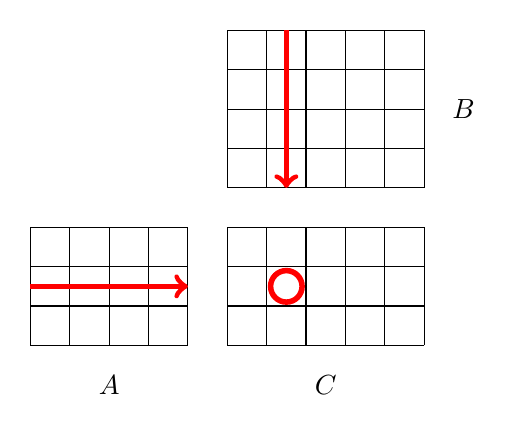
\begin{tikzpicture}[scale=0.5]
\draw (0,0) grid (4,3);
\draw (5,0) grid (10,3);
\draw (5,4) grid (10,8);

\node at (2,-1) {$A$};
\node at (7.5,-1) {$C$};
\node at (11,6) {$B$};

\draw[thick,->,red,line width=2pt] (0,1.5) -- (4,1.5);
\draw[thick,->,red,line width=2pt] (6.5,8) -- (6.5,4);
\draw[thick,red,line width=2pt] (6.5,1.5) circle (0.4);
\end{tikzpicture}
\end{center}

Esimerkiksi

\[
 \begin{bmatrix}
  1 & 4 \\
  3 & 9 \\
  8 & 6 \\
 \end{bmatrix}
\cdot
 \begin{bmatrix}
  1 & 6 \\
  2 & 9 \\
 \end{bmatrix}
=
 \begin{bmatrix}
  1 \cdot 1 + 4 \cdot 2 & 1 \cdot 6 + 4 \cdot 9 \\
  3 \cdot 1 + 9 \cdot 2 & 3 \cdot 6 + 9 \cdot 9 \\
  8 \cdot 1 + 6 \cdot 2 & 8 \cdot 6 + 6 \cdot 9 \\
 \end{bmatrix}
=
 \begin{bmatrix}
  9 & 42 \\
  21 & 99 \\
  20 & 102 \\
 \end{bmatrix}.
\]

Matriisien kertolasku ei ole vaihdannainen,
eli ei ole voimassa $A \cdot B = B \cdot A$.
Kuitenkin matriisien kertolasku
on liitännäinen, eli on voimassa $A \cdot (B \cdot C)=(A \cdot B) \cdot C$.
Lukua 1 vastaa ykkösmatriisi $I$,
jolle pätee $A \cdot I = A$ ja $I \cdot A = A$.
Ykkösmatriisi on neliömatriisi, jossa $I[i,j]=1$,
jos $i=j$, ja muuten $I[i,j]=0$.

Esimerkiksi

\[
 \begin{bmatrix}
  1 & 0 \\
  0 & 1 \\
 \end{bmatrix}
\cdot
 \begin{bmatrix}
  1 & 6 \\
  2 & 9 \\
 \end{bmatrix}
=
 \begin{bmatrix}
  1 & 6 \\
  2 & 9 \\
 \end{bmatrix}
\cdot
 \begin{bmatrix}
  1 & 0 \\
  0 & 1 \\
 \end{bmatrix}
=
 \begin{bmatrix}
  1 & 6 \\
  2 & 9 \\
 \end{bmatrix}
\]

Kertolaskun määritelmästä seuraa $O(n^3)$-algoritmi
kahden $n \times n$ -kokoisen
neliömatriisin kertomiseen:

\begin{lstlisting}
for (int i = 1; i <= n; i++) {
    for (int j = 1; j <= n; j++) {
        for (int k = 1; k <= n; k++) {
            C[i][j] += A[i][k]*B[k][j];
        }
    }
}
\end{lstlisting}

Tämä algoritmi on riittävän nopea kisakoodauksessa,
mutta myös tehokkaampia algoritmeja on olemassa.
Tällä hetkellä tehokkain tunnettu
algoritmi on vaativuudeltaan $O(n^{2{,}3728639})$.
Tämä algoritmi on kuitenkin hyvin monimutkainen
ja sen vakiokertoimet ovat suuret.

\subsubsection{Potenssilasku}

Matriisin $A$ potenssilasku $A^k$ on
määritelty, jos $A$ on neliömatriisi kokoa $n \times n$.
Määritelmä nojautuu kertolaskuun:

\[ A^k = \underbrace{A \cdot A \cdot A \cdots A}_{\textrm{$k$ kertaa}} \]

Esimerkiksi

\[
 \begin{bmatrix}
  2 & 5 \\
  1 & 4 \\
 \end{bmatrix}^3 =
 \begin{bmatrix}
  2 & 5 \\
  1 & 4 \\
 \end{bmatrix} \cdot
 \begin{bmatrix}
  2 & 5 \\
  1 & 4 \\
 \end{bmatrix} \cdot
 \begin{bmatrix}
  2 & 5 \\
  1 & 4 \\
 \end{bmatrix} =
 \begin{bmatrix}
  48 & 165 \\
  33 & 114 \\
 \end{bmatrix}.
\]

Potenssilasku $A^k$ muodostuu $k$ kertolaskusta,
joten aikavaativuus on $O(n^3 k)$.
Tätä on mahdollista tehostaa soveltamalla
tehokasta potenssilaskua (luku 21.2),
jolloin aikavaativuus on vain $O(n^3 \log k)$.
Esimerkiksi
\[
 \begin{bmatrix}
  2 & 5 \\
  1 & 4 \\
 \end{bmatrix}^8 =
 \begin{bmatrix}
  2 & 5 \\
  1 & 4 \\
 \end{bmatrix}^4 \cdot
 \begin{bmatrix}
  2 & 5 \\
  1 & 4 \\
 \end{bmatrix}^4.
\]


\subsubsection{Determinantti}

Matriisin $A$ determinantti $\det(A)$
on määritelty, jos $A$ on neliömatriisi.
Jos $A$ on kokoa $1 \times 1$,
niin $\det(A)=A[1,1]$.
Muuten determinaatti lasketaan rekursiivisesti
kaavalla

\[\det(A)=\sum_{i=1}^n A[1,i] \cdot det(A') \cdot (-1)^{i+1},\]

missä $A'$ tarkoittaa matriisia $A$,
josta on poistettu rivi 1 ja sarake $i$.
Huomaa myös, että $(-1)^{i+1}$ on $1$,
jos $i$ on pariton, ja muuten $-1$.

Esimerkiksi

\[
\det(
 \begin{bmatrix}
  3 & 4 \\
  1 & 6 \\
 \end{bmatrix}
) = 3 \cdot 6 - 4 \cdot 1 = 14 
\]

ja

\[
\det(
 \begin{bmatrix}
  2 & 4 & 3 \\
  5 & 1 & 6 \\
  7 & 2 & 4 \\
 \end{bmatrix}
) = 
2 \cdot
\det(
 \begin{bmatrix}
  1 & 6 \\
  2 & 4 \\
 \end{bmatrix}
)
-4 \cdot
\det(
 \begin{bmatrix}
  5 & 6 \\
  7 & 4 \\
 \end{bmatrix}
)
+3 \cdot
\det(
 \begin{bmatrix}
  5 & 1 \\
  7 & 2 \\
 \end{bmatrix}
) = 81.
\]

Determinantti kertoo, onko matriisille
$A$ olemassa käänteismatriisia
$A^{-1}$, jolle pätee $A \cdot A^{-1} = I$.
Osoittautuu, että käänteismatriisi on olemassa
tarkalleen silloin, kun $\det(A) \neq 0$.
Esimerkiksi

\[
\underbrace{
 \begin{bmatrix}
  3 & 4 \\
  1 & 6 \\
 \end{bmatrix}
}_{A}
\cdot
\underbrace{
 \begin{bmatrix}
  \frac{3}{7} & -\frac{2}{7} \\
  -\frac{1}{14} & \frac{3}{14} \\
 \end{bmatrix}
}_{A^{-1}}
=
\underbrace{
 \begin{bmatrix}
  1 & 0 \\
  0 & 1 \\
 \end{bmatrix}
}_{I}.
\]

\section{Dynaaminen ohjelmointi}

Matriisien ja tehokkaan potenssilaskun hyötynä on,
että tietyt dynaamisen ohjelmoinnin ratkaisut
voi esittää matriisimuodossa.
Niinpä tehokkaan potenssilaskun avulla
aikavaativuuden lineaarisesta
kertoimesta tulee logaritminen.

Tarkastellaan esimerkkinä tästä
Fibonaccin lukujen laskemista.
Tavallinen rekursiivinen kaava on:
\[
\begin{array}{lcl}
F_0 & = & 0 \\
F_1 & = & 1 \\
F_n & = & F_{n-2}+F_{n-1} \\
\end{array}
\]

Matriisimuodossa asian voi esittää näin:

\[
X=\left( \begin{array}{cc}
0 & 1 \\
1 & 1 \end{array} \right)
\]
\[
X \cdot
\left( \begin{array}{c}
F_k \\
F_{k+1} \end{array} \right)
=
\left( \begin{array}{c}
F_{k+1} \\
F_{k+2} \end{array} \right)
\]

Ideana on,
että jos $2 \times 1$ -matriisissa
on peräkkäiset Fibonaccin luvut $F_k$ ja $F_{k+1}$,
kertominen matriisilla $X$
tuottaa uuden matriisin,
jossa on peräkkäiset Fibonaccin luvut
$F_{k+1}$ ja $F_{k+2}$. Esimerkiksi
\[
X\cdot
\left( \begin{array}{c}
F_5 \\
F_6 \end{array} \right)
= 
\left( \begin{array}{cc}
0 & 1 \\
1 & 1 \end{array} \right)
\cdot
\left( \begin{array}{c}
5 \\
8 \end{array} \right)
= \left( \begin{array}{c}
0\cdot5+1\cdot8 \\
1\cdot5+1\cdot8 \end{array} \right)
= \left( \begin{array}{c}
8 \\
13 \end{array} \right)
= \left( \begin{array}{c}
F_6 \\
F_7 \end{array} \right).
\]

Tämän ansiosta arvon $F_n$ sisältävän matriisin saa laskettua

\[
\left( \begin{array}{c}
F_n \\
F_{n+1} \end{array} \right)
= X^n\cdot
\left( \begin{array}{c}
F_0 \\
F_1 \end{array} \right)
=
\left( \begin{array}{cc}
0 & 1 \\
1 & 1 \end{array} \right)^n
\cdot
\left( \begin{array}{c}
0 \\
1 \end{array} \right).
\]

Matriisin potenssilasku onnistuu ajassa $O(\log n)$,
joten tällä tekniikalla Fibonaccin luvun $F_n$
pystyy laskemaan ajassa $O(\log n)$.
Samaa ideaa voi myös soveltaa aina,
kun rekursiivisen funktion seuraava arvo
saadaan laskemalla yhteen kiinteä määrä
edellisiä arvoja sopivilla kertoimilla.

\section{Verkko matriisina}

Matriisin potenssilaskulla
on mielenkiintoinen vaikutus
painottoman
verkon vierusmatriisin sisältöön.
Kun $V$ on vierusmatriisi,
jossa jokainen arvo on 0 tai 1,
niin $V^n$ kertoo,
montako $n$:n pituista polkua
eri solmuista on toisiinsa.

Esimerkiksi verkon
\\
\begin{center}
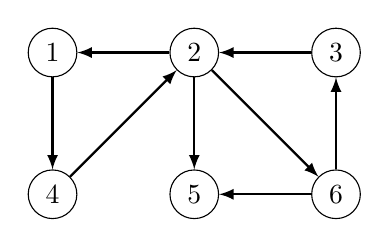
\begin{tikzpicture}[scale=0.9]
\node[draw, circle] (1) at (1,3) {$1$};
\node[draw, circle] (2) at (1,1) {$4$};
\node[draw, circle] (3) at (3,3) {$2$};
\node[draw, circle] (4) at (5,3) {$3$};
\node[draw, circle] (5) at (3,1) {$5$};
\node[draw, circle] (6) at (5,1) {$6$};

\path[draw,thick,->,>=latex] (1) -- (2);
\path[draw,thick,->,>=latex] (2) -- (3);
\path[draw,thick,->,>=latex] (3) -- (1);
\path[draw,thick,->,>=latex] (4) -- (3);
\path[draw,thick,->,>=latex] (3) -- (5);
\path[draw,thick,->,>=latex] (3) -- (6);
\path[draw,thick,->,>=latex] (6) -- (4);
\path[draw,thick,->,>=latex] (6) -- (5);
\end{tikzpicture}
\end{center}

vierusmatriisi on

\[
V=
\left( \begin{array}{cccccc}
0 & 0 & 0 & 1 & 0 & 0 \\
1 & 0 & 0 & 0 & 1 & 1 \\
0 & 1 & 0 & 0 & 0 & 0 \\
0 & 1 & 0 & 0 & 0 & 0 \\
0 & 0 & 0 & 0 & 0 & 0 \\
0 & 0 & 1 & 0 & 1 & 0 \end{array} \right).
\]

Nyt esimerkiksi matriisi $V^3$ kertoo
3:n pituisten polkujen määrät:
\[
V^3=
\left( \begin{array}{cccccc}
1 & 0 & 0 & 0 & 1 & 1 \\
0 & 2 & 0 & 0 & 0 & 0 \\
0 & 0 & 1 & 1 & 1 & 0 \\
0 & 0 & 1 & 1 & 1 & 0 \\
0 & 0 & 0 & 0 & 0 & 0 \\
1 & 0 & 0 & 0 & 1 & 1 \end{array} \right).
\]

Esimerkiksi $(V^3)_{1,5}=1$,
koska solmusta 1 pääsee solmuun 5
kulkemalla polkua $1 \rightarrow 4 \rightarrow 2 \rightarrow 5$.
Vastaavasti $(V^3)_{2,2}=2$,
koska solmusta 2 pääsee itseensä
kulkemalla polkuja
$2 \rightarrow 1 \rightarrow 4 \rightarrow 2$
sekä $2 \rightarrow 6 \rightarrow 3 \rightarrow 2$.

Samantapaista ideaa voi käyttää myös
laskemaan painotetussa verkossa,
mikä on lyhin $k$ kaaren pituinen polku
kunkin solmun välillä.
Tämän saavuttamiseksi riittää muuttaa matriisikertolaskun
kaavassa yhteenlasku minimiksi
ja kertolasku yhteenlaskuksi,
jolloin kaavasta tulee

\[
(AB)_{i,j} = \min_{k=1}^n (A_{i,k}+B_{k,j}).
\]

